% Source - https://tex.stackexchange.com/a/764079

\documentclass[varwidth,border=2pt]{standalone}
\usepackage{tikz}
\usetikzlibrary{nfold, intersections, spath3, decorations.markings}
\tikzset{
    place ortho/.style 2 args={
        preaction={
        path only,
        decorate,
        decoration={
            name=markings,
            mark=at position #1 with {\path[overlay, spath/save global=o#2] (down:5mm) -- (up:5mm);}
            }
        }
    }
}
\makeatletter
    \tikzset{offset/.code=\tikz@addoption{\pgfgetpath\tikz@temp\pgfsetpath\pgfutil@empty\pgfoffsetpath\tikz@temp{#1}}}
\makeatother
\newcommand*\spathset{\pgfqkeys{/tikz/spath}}
\begin{document}
    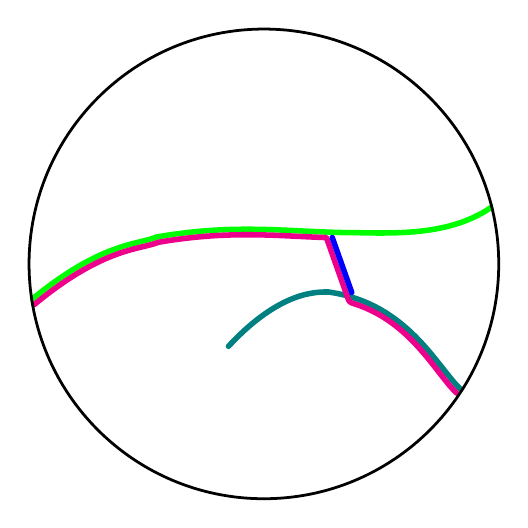
\begin{tikzpicture}[
        line cap=round, line join=round,
        scale=3, line width=2pt,
        make path/.style 2 args={
            color=#1, spath/save=p#1, 
            place ortho={#2}{#1}
        }]
        \clip circle[radius=1];
        \draw[make path={green}{0.65}] (-0.988,-0.155)
        .. controls (-0.689,0.093) and (-0.531,0.081) .. (-0.454,0.114)
        .. controls (-0.099,0.175) and (0.111,0.132) .. (0.402,0.132)
        .. controls (0.617,0.127) and (0.819,0.132) .. (0.98,0.252);
        \draw[make path={teal}{0.5}] (-0.15,-0.349)
        .. controls (0.072,-0.109) and (0.231,-0.119) .. (0.274,-0.119)
        .. controls (0.607,-0.167) and (0.729,-0.431) .. (0.832,-0.53) ;
        \spathset{
            split at intersections with={pgreen}{ogreen}, remove components={pgreen}{2},
            split at intersections with={pteal}{oteal}, remove components={pteal}{1},
        }
        \draw[magenta, spath/use={pgreen}] -- (spath cs:pteal 0) [spath/use={pteal, weld}, offset=+-\pgflinewidth];
        \draw[blue, shorten >=+\pgflinewidth, shorten <=+\pgflinewidth] (spath cs:pgreen 1) -- (spath cs:pteal 0);
        \draw circle[radius=1];
    \end{tikzpicture}

    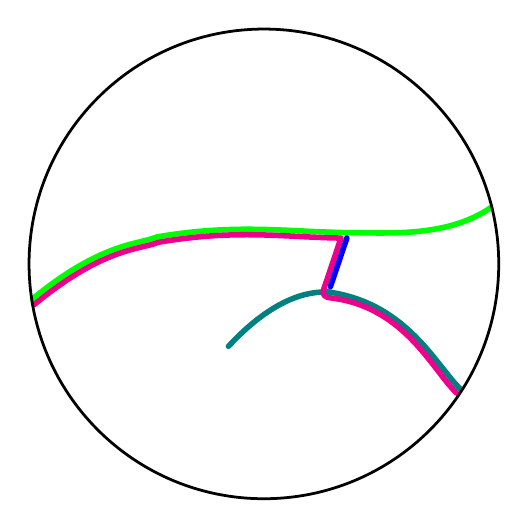
\begin{tikzpicture}[
        line cap=round, line join=round,
        scale=3, line width=2pt,
        make path/.style={color=#1, spath/save=p#1}
    ]
    \clip circle[radius=1];
    \draw[make path=green] (-0.988,-0.155)
    .. controls (-0.689,0.093) and (-0.531,0.081) .. (-0.454,0.114)
    .. controls (-0.099,0.175) and (0.111,0.132) .. (0.402,0.132)
    .. controls (0.617,0.127) and (0.819,0.132) .. (0.98,0.252);
    \draw[make path=teal] (-0.15,-0.349)
    .. controls (0.072,-0.109) and (0.231,-0.119) .. (0.274,-0.119)
    .. controls (0.607,-0.167) and (0.729,-0.431) .. (0.832,-0.53) ;
    \spathset{
        split at keep start={pgreen}{0.65},
        split at keep end={pteal}{0.5},
    }
    \draw[magenta, spath/use={pgreen}] -- (spath cs:pteal 0) [spath/use={pteal, weld}, offset=+-\pgflinewidth];
    \draw[blue, shorten >=+\pgflinewidth, shorten <=+\pgflinewidth] (spath cs:pgreen 1) -- (spath cs:pteal 0);
    \draw circle[radius=1];
\end{tikzpicture}
\end{document}
